\let\negmedspace\undefined
\let\negthickspace\undefined
\documentclass[journal,12pt,onecolumn]{IEEEtran}
\usepackage{cite}
\usepackage{amsmath,amssymb,amsfonts,amsthm}
\usepackage{algorithmic}
\usepackage{graphicx}
\graphicspath{{./figs/}}
\usepackage{textcomp}
\usepackage{xcolor}
\usepackage{txfonts}
\usepackage{listings}
\usepackage{enumitem}
\usepackage{mathtools}
\usepackage{gensymb}
\usepackage{comment}
\usepackage{caption}
\usepackage[breaklinks=true]{hyperref}
\usepackage{tkz-euclide} 
\usepackage{listings}
\usepackage{gvv}                                        
%\def\inputGnumericTable{}                                 
\usepackage[latin1]{inputenc}     
\usepackage{xparse}
\usepackage{color}                                            
\usepackage{array}                                            
\usepackage{longtable}                                       
\usepackage{calc}                                             
\usepackage{multirow}
\usepackage{multicol}
\usepackage{hhline}                                           
\usepackage{ifthen}                                           
\usepackage{lscape}
\usepackage{tabularx}
\usepackage{array}
\usepackage{float}
%\newtheorem{theorem}{Theorem}[section]
%\newtheorem{theorem}{Theorem}[section]
%\newtheorem{problem}{Problem}
%\newtheorem{proposition}{Proposition}[section]
%\newtheorem{lemma}{Lemma}[section]
%\newtheorem{corollary}[theorem]{Corollary}
%\newtheorem{example}{Example}[section]
%\newtheorem{definition}[problem]{Definition}

\begin{document}

%\textbf{\Large 4.8.23} \\
%\textbf{\large AI25BTECH11027 - NAGA BHUVANA} \\
\title{4.8.23}
\author{AI25BTECH11027 - NAGA BHUVANA}
% \maketitle
% \newpage
% \bigskip
%\begin{document}
{\let\newpage\relax\maketitle}
%\renewcommand{\thefigure}{\theenumi}
%\renewcommand{\thetable}{\theenumi}
\noindent
		\textbf{Question:}\\
Find the values of $\lambda$,for which the distance of point $(2,1,\lambda)$ from plane $3x+5y+4z=11$ is $2\sqrt{2}$ units.\\
\textbf{Solution:}\\
The normal vector of the plane is $\myvec{3\\5\\4}$ and $\vec{P}=\myvec{2\\1\\\lambda}$\\
The equation of the plane be $\vec{n}^T\vec{x}=c$
\begin{align}
    distance=\frac{|\vec{n}^T\vec{p}-11|}{\|\vec{n}\|}
\end{align}
\begin{align}
    2\sqrt{2}=\frac{|\myvec{3&5&4}\myvec{2\\1\\\lambda}-11|}{5\sqrt{2}}
\end{align}
        \begin{align}
            \frac{|4\lambda|}{5\sqrt{2}}=2\sqrt{2}
        \end{align}
        \begin{align}
            |4\lambda|=20
        \end{align}
        \begin{align}
            4\lambda=20  \quad \text{or} \quad -4\lambda=-20
        \end{align}
        \begin{align}
            \lambda=5 \quad \text{or} \quad \lambda=-5
        \end{align}
        $\therefore $The values of $\lambda=5$ or $-5$
	\begin{figure}[H]
		\centering
		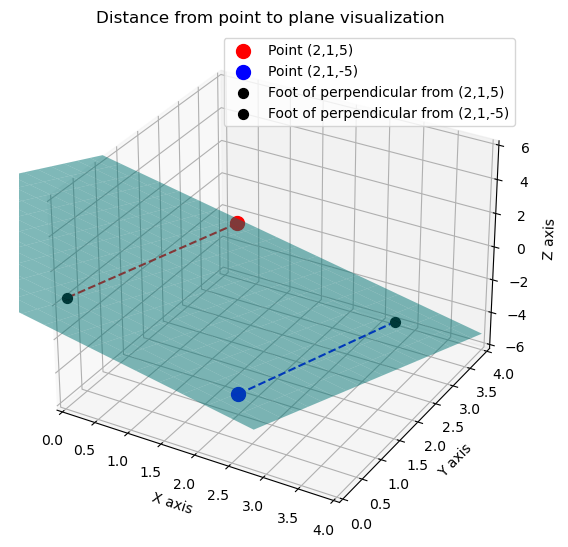
\includegraphics[width=0.7\linewidth]{figs/fig1.png}
		\caption{}
		\label{fig}
	\end{figure}
\end{document}
